
\subsection{\textit{Kygo}}
  Partamos por crear un paquete \texttt{cl.ravenhill.kygo} en el directorio \url{src/main/kotlin}.

  Ahora debemos iniciar el repositorio de \textit{Git} en el directorio del proyecto.
  Para esto primero hagamos click derecho en el directorio del proyecto y seleccionemos la opción
  \textit{Copy Path/Reference\dots} (\cref{fig:copy-path}).
  Luego, en la ventana que se abrió, hagamos click en el botón \textit{Absolute Path} 
  (\cref{fig:abs-path}).

  \begin{figure}[H]
    \centering
    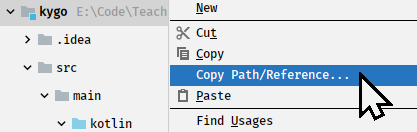
\includegraphics[width=0.5\textwidth]{img/oop/principios/vcs/copy-path.png}
    \caption{Copiando la ruta del proyecto}
    \label{fig:copy-path}
  \end{figure}

  \begin{figure}[H]
    \centering
    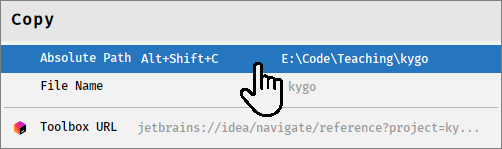
\includegraphics[width=0.5\textwidth]{img/oop/principios/vcs/abs-path.png}
    \caption{Copiando la ruta absoluta del proyecto}
    \label{fig:abs-path}
  \end{figure}

  Ahora abramos una terminal y ejecutemos el siguiente comando:

  \begin{defaultbox}[Windows]
    \begin{powershell}
      Get-Clipboard | Set-Location
      git init
    \end{powershell}
  \end{defaultbox}

  \begin{defaultbox}[Linux]
    \begin{bash}
      cd $(xclip -o -selection clipboard)
      git init
    \end{bash}
  \end{defaultbox}

  \begin{defaultbox}[MacOS]
    \begin{bash}
      cd $(pbpaste)
      git init
    \end{bash}
  \end{defaultbox}

  Veamos lo que está pasando en el comando anterior:
  \begin{itemize}
    \item Primero tomamos el contenido del portapapeles y lo usamos como argumento al comando 
      \texttt{cd}\footnote{Change directory}/\texttt{Set-Location} para cambiar el directorio actual a la ruta del proyecto.
    \item Luego ejecutamos el comando \idx{\texttt{git init}}.
      El comando \texttt{git init} inicializa un repositorio de \textit{Git} en el directorio
      actual, esto significa que \textit{Git} comenzará a monitorear los cambios que se realicen
      en el directorio actual.
  \end{itemize}

  Nos queda verificar que el repositorio de \textit{Git} se haya creado correctamente.
  Para esto ejecutemos el comando \idx{\texttt{git status}} (nuestro otro mejor amigx), esto nos entregará
  un mensaje como el siguiente:

  \begin{minted}{text}
    On branch master

    No commits yet

    Untracked files:
      (use "git add <file>..." to include in what will be committed)
            .idea/
            kygo.iml

    nothing added to commit but untracked files present (use "git add" to track)
  \end{minted}

  Aquí lo que nos está diciendo \textit{Git} es que existen archivos que no están siendo 
  monitoreados y que, por lo tanto, no forman parte del repositorio.

  Podríamos agregar estos archivos directamente al repositorio, pero en general no es una buena 
  idea.
  Como dijimos, esos elementos son de configuración y si estamos trabajando con otras personas
  podría causar problemas si todos tienen configuraciones diferentes.
  Por esto nos gustaría poder no sólo no agregarlos, sino que asegurarnos de que nunca\footnote{
    Existen formas de agregarlos de todos modos, pero por qué quieres hacer eso \texttt{D:}
  } 
  se agreguen.

  Para esto debemos crear un archivo llamado \idx{\texttt{.gitignore}} en el directorio raíz del 
  proyecto.
  Este archivo contiene una lista de patrones que \textit{Git} usará para ignorar archivos
  que coincidan con esos patrones.
  En nuestro caso, vamos a ignorar todos los archivos que estén en el directorio \texttt{.idea/} y
  el archivo \texttt{kygo.iml}.
  Para esto, abramos el archivo \texttt{.gitignore} y agreguemos las siguientes líneas:

  \begin{minted}{text}
    .idea/
    kygo.iml
  \end{minted}

  Ahora, si volvemos a ejecutar el comando \texttt{git status} veremos que el único archivo que
  \textit{Git} nos está indicando que no está siendo monitoreado es el archivo \texttt{.gitignore}.

  Digámosle ahora a \textit{Git} que empiece a monitorear el archivo \texttt{.gitignore}.
  Para esto ejecutemos el comando \idx{\texttt{git add .gitignore}}.
  Este comando le dice a \textit{Git} que agregue el archivo \texttt{.gitignore} al repositorio.
